\documentclass[12pt]{kiarticle} % You can learn about my document class "kiarticle" and install it to your device by following the link: https://github.com/Kiarendil/toolkitex
\graphicspath{{pictures/}}
\DeclareGraphicsExtensions{.pdf,.png,.jpg,.eps}
%%%
\pagestyle{fancy}
\fancyhf{}
%\renewcommand{\headrulewidth}{ 0.1mm }
\renewcommand{\footrulewidth}{ .0em }
\fancyfoot[C]{\texttt{\textemdash~\thepage~\textemdash}}
\fancyhead[L]{Лабораторная работа № 4.2 \hfil}
\fancyhead[R]{\hfil Иванов Кирилл, 625 группа }
\usepackage{multirow} % Слияние строк в таблице
\newcommand
{\un}[1]
{\ensuremath{\text{#1}}}
\newcommand{\eds}{\ensuremath{ \mathscr{E}}}
\newcommand{\be}{\ensuremath{\beta}}
\usepackage{tikz}
%%% Работа с таблицами
\usepackage{array,tabularx,tabulary,booktabs} % Дополнительная работа с таблицами
\usepackage{longtable}  % Длинные таблицы
\usepackage{multirow} % Слияние строк в таблице

\begin{document}
	
	\begin{titlepage}
		\begin{center}
			\large 	Московский физико-технический институт \\
			(государственный университет) \\
			Факультет общей и прикладной физики \\
			\vspace{0.2cm}
			
			\vspace{4.5cm}
			Лабораторная работа № 4.2 \\ \vspace{0.2cm}
			\large (Общая физика: квантовая физика) \\ \vspace{0.2cm}
			\LARGE \textbf{ Исследование энергетического спектра \be-частиц
				и определение их максимальной энергии при помощи
				магнитного спектрометра }
		\end{center}
		\vspace{2.3cm} \large
		
		\begin{center}
			Работу выполнил: \\
			Иванов Кирилл,
			625 группа
			\vspace{10mm}		
			
		\end{center}
		
		\begin{center} \vspace{60mm}
			г. Долгопрудный \\
			2018 год
		\end{center}
	\end{titlepage}


\paragraph*{Цель работы:} С помощью магнитного спектрометра исследовать энергетический спектр $\beta$ - частиц при распаде ядер $^{137}$Cs  и определить их максимальную энергию.

\section{Теоретическое введение} 

Бета-распадом называется самопроизвольное превращение ядер, при котором их массовое число не изменяется, а заряд увеличивается или уменьшается на единицу. Бета-активные ядра встречаются во всей области значений массового числа A, начиная от единицы (свободный нейтрон) и кончая самыми тяжелыми ядрами. Период полураспада $\beta$ - активных ядер изменяется от ничтожных долей секунды до $10^{18}$ лет. Выделяющаяся при единичном акте $\beta$ - распада энергия варьируется от 18 кэВ до 13,4 МэВ.

В данной работе мы будем иметь дело с электронным распадом

\begin{equation}\label{}
^A_ZX \rightarrow ^{\; \; \; \; \: A}_{Z+1}X + e^- + \widetilde{\nu}
\end{equation}

при котором кроме электрона испускается антинейтрино. Освобождающаяся при $\beta$-распаде энергия делится между электроном, антинейтрино и дочерним ядром, однако доля энергии, передаваемой ядру, исчезающе мала по сравнению с энергией, уносимой электроном и антинейтрино. Практически можно считать, что эти две частицы делят между собой всю освобождающуюся энергию. Поэтому электроны могут иметь любое значение энергии  от нулевой до некоторой максимальной, которая равна энергии, освобождающейся при $\beta$-распаде, являющейся важной физической величиной.

Вероятность $ dw $ того, что при распаде электрон вылетит с импульсом в интервале $d^3p$, а антинейтрино с импульсом в интервале $d^3k$, пропорциональна произведению этих дифференциалов. Но мы должны еще учесть закон сохранения энергии, согласно которому импульсы $ p $ и $ k $ электрона и антинейтрино связаны соотношением

\begin{equation}
E_e - E - ck = 0,
\end{equation}

где $E_e$ - максимальная энергия электрона, кинетическая энергия электрона $ E $ связана с его импульсом обычным релятивистским соотношением

\begin{equation}
E = c\sqrt{p^2 + m^2c^2} - mc^2,
\end{equation}

а через $ ck $ обозначена энергия антинейтрино с импульсом $ k $. Условие можно учесть введением в выражение для $ dw $ $\delta$ - функции
\begin{equation}
\delta (E_e - E - ck).
\end{equation}

Таким образом, вероятность $ dw $ может быть записана в виде

\begin{equation}\label{dw}
dw = D \delta (E_e - E - ck)d^3 p d^3 k = D \delta (E_e - E - ck)p^2dpk^2dkd{\Omega}_ed{\Omega}_{\widetilde{\nu}},
\end{equation}

где $ D $ --- некоторый коэффициент пропорциональности, $d\Omega_e$ , $d\Omega_{\widetilde{\nu}}$ --- элементы телесных углов направлений вылета электрона и нейтрино. Вероятность $ dw $ непосредственно связана с $\beta$-спектром, поскольку для большого числа $N_0$ распадов число $dN$ распадов с вылетом электрона и антинейтрино с импульсом соответственно от $ p $ до $ p + dp $ и от
$ k $ до $ k + d $k определяется соотношением

\begin{equation}\label{dn = n_0 dw}
dN = N_0 dw  
\end{equation}

Коэффициент $ D $ в формуле \eqref{dw} можно считать для рассматриваемых нами так называемых разрешенных фермиевских типов распадов с хорошей точностью константой (разрешенными называются такие переходы, при которых не изменяются ни момент, ни четность состояния ядра). В этом случае величину $ dw $ из \eqref{dn = n_0 dw} можно проинтегрировать по всем углам и по абсолютному значению импульса нейтрино.

После умножения на полное число распадов $ N $ проинтегрированное выражение приобретает смысл числа электронов $ dN $, вылетающих из ядра с импульсом, абсолютная величина которого лежит между $ p $ и$  p + dp $:

\begin{equation}\label{dN}
dN = \dfrac{16\pi^2 N_0}{c^2}Dp^2(E_e - E)^2dp.
\end{equation}

Чтобы получить распределение электронов по энергиям, надо в \eqref{dN} перейти от $ dp $ к $ dE $:

\begin{equation}
dE = \dfrac{c^2p}{E + mc^2}dp,
\end{equation}

после чего выражающая форму $\beta$ --- спектра величина $ N(E) = dN/dE $
приобретает вид

\begin{equation}\label{dN/dE big}
\dfrac{dN}{dE} = N_0Bcp(E + mc^2)(E_e - E)^2 = N_0B\sqrt{E(E + 2mc^2)}(E_e - E)^2(E + mc^2)
\end{equation}

где $B = (16\pi^2/c^4)D$. В нерелятивистском приближении, которое и имеет место с нашем случае, выражение \eqref{dN/dE big} упрощается, и мы имеем

\begin{equation}\label{dN/dE}
\dfrac{dN}{dE} \approx \sqrt{E}(E_e - E)^2.
\end{equation}

\begin{wrapfigure}[12]{l}{0.35\linewidth}
	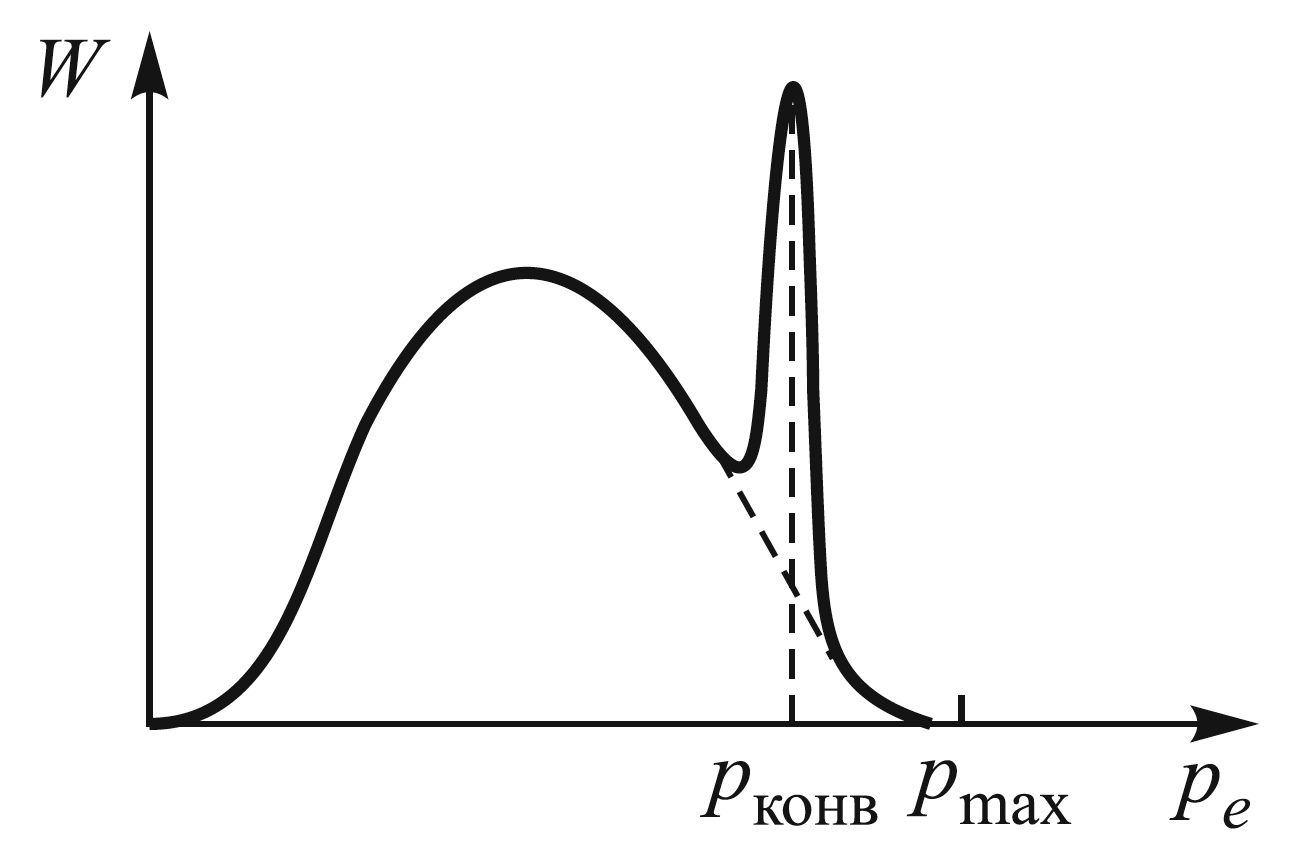
\includegraphics[width=\linewidth]{spektr}
	\caption{Форма спектра \be-частиц
		при разрешенных переходах}
	\label{ris spetr}
\end{wrapfigure}


Выражение \eqref{dN/dE} приводит к спектру, имеющему вид широкого колокола (рис \ref{ris spetr}). Кривая плавно отходит от нуля и столь же плавно, по параболе, касается оси абсцисс в области максимальной энергии электронов $E_e$. 

Дочерние ядра, возникающие в результате $\beta$-распада, нередко оказываются возбужденными. Возбужденные ядра отдают свою энергию либо излучая $\gamma$-квант (энергия которого равна разности энергий начального и конечного уровней), либо передавая избыток энергии одному из электронов с внутренних оболочек атома. Излучаемые в таком процессе электроны имеют строго определенную энергию и называются конверсионными.

Конверсия чаще всего происходит на оболочках $ K $ или $ L $. На спектре, представленном на рис. \ref{ris spetr}, видна монохроматическая линия, вызванная электронами конверсии. Ширина этой линии в нашем случае является чисто аппаратурной, по ней можно оценить разрешающую силу спектрометра.


\section{Экспериментальная установка}
	
	Для определения энергии $\beta$-частиц в работе используется магнитный спектрометр, схема которого показана на рисунке \ref{pic:scheme} слева. Электроны испускаются радиоактивным источником и попадают в магнитное поле катушки, ось которой параллельна $OZ$. Траектории электронов сходятся в одной точке --- фокусе, где и установлен сцинтилляционный счетчик, сигналы которого усиливаются фотоумножителем и регистрируются пересчетным прибором. Фокусное расстояние $f$ магнитной линзы связано с током в катушке $I$ и импульсом $p_e$ регистрируемых частиц следующим образом:
	
	\[ \frac{1}{f} \propto \frac{I^2}{p_e^2} \]  
	
	При неизменной геометрии установки, увеличивая и уменьшая силу тока, можно фокусировать электроны разных импульсов, причем 
	
	\begin{equation}\label{k}
	p_e = kI,
	\end{equation}
	
	 где $k$ --- коэффициент пропорциональности, являющийся параметром установки.

	\begin{figure}[h]
	\centering
	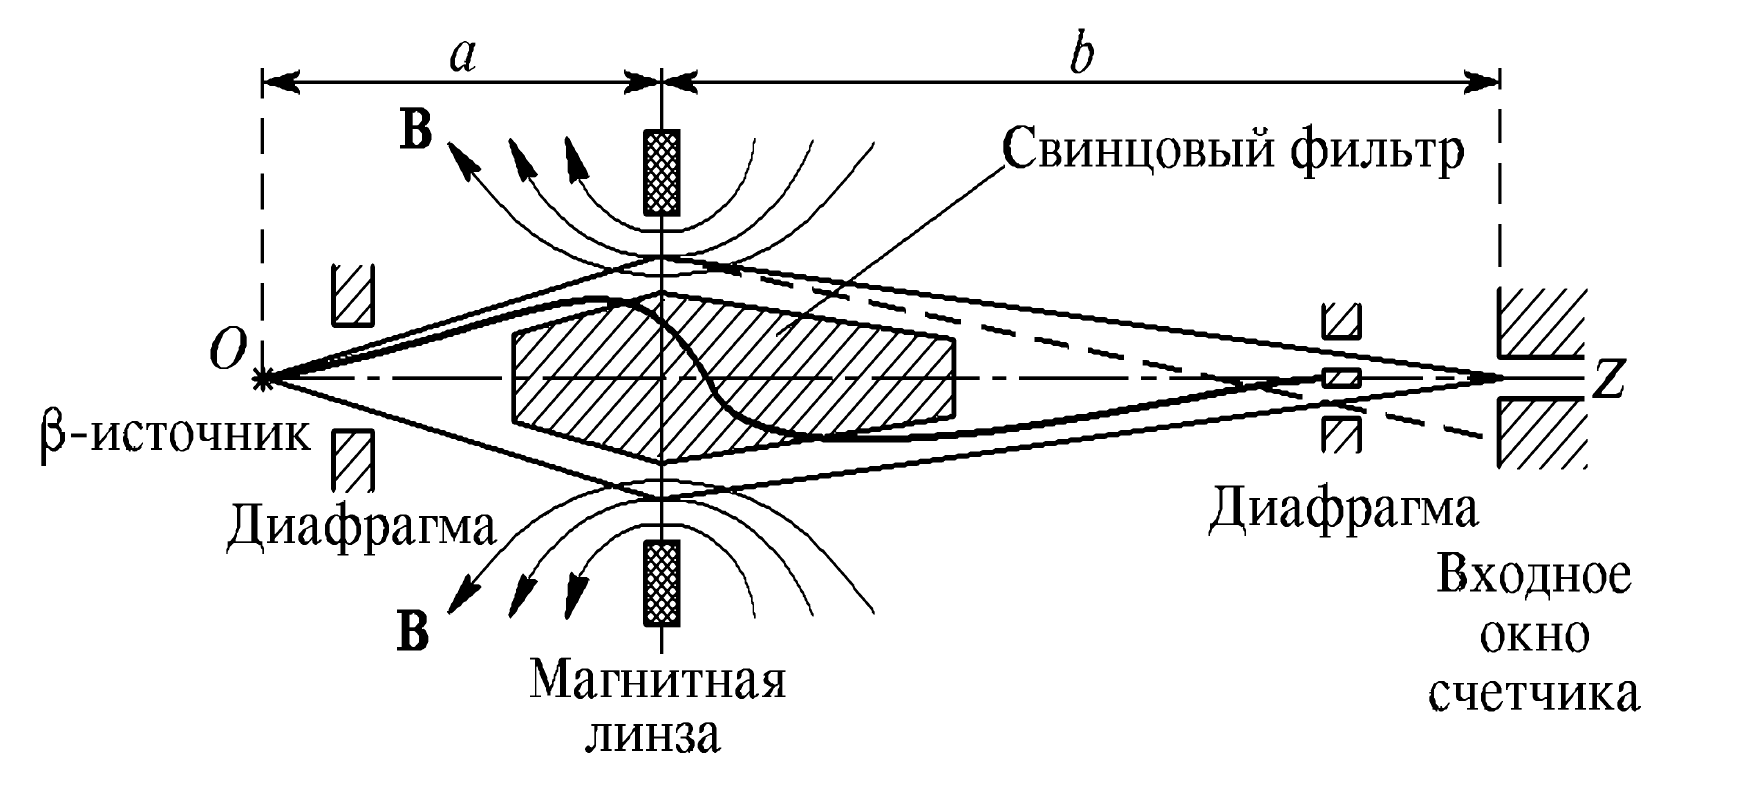
\includegraphics[width=0.48\textwidth]{lab}
	\hfill
	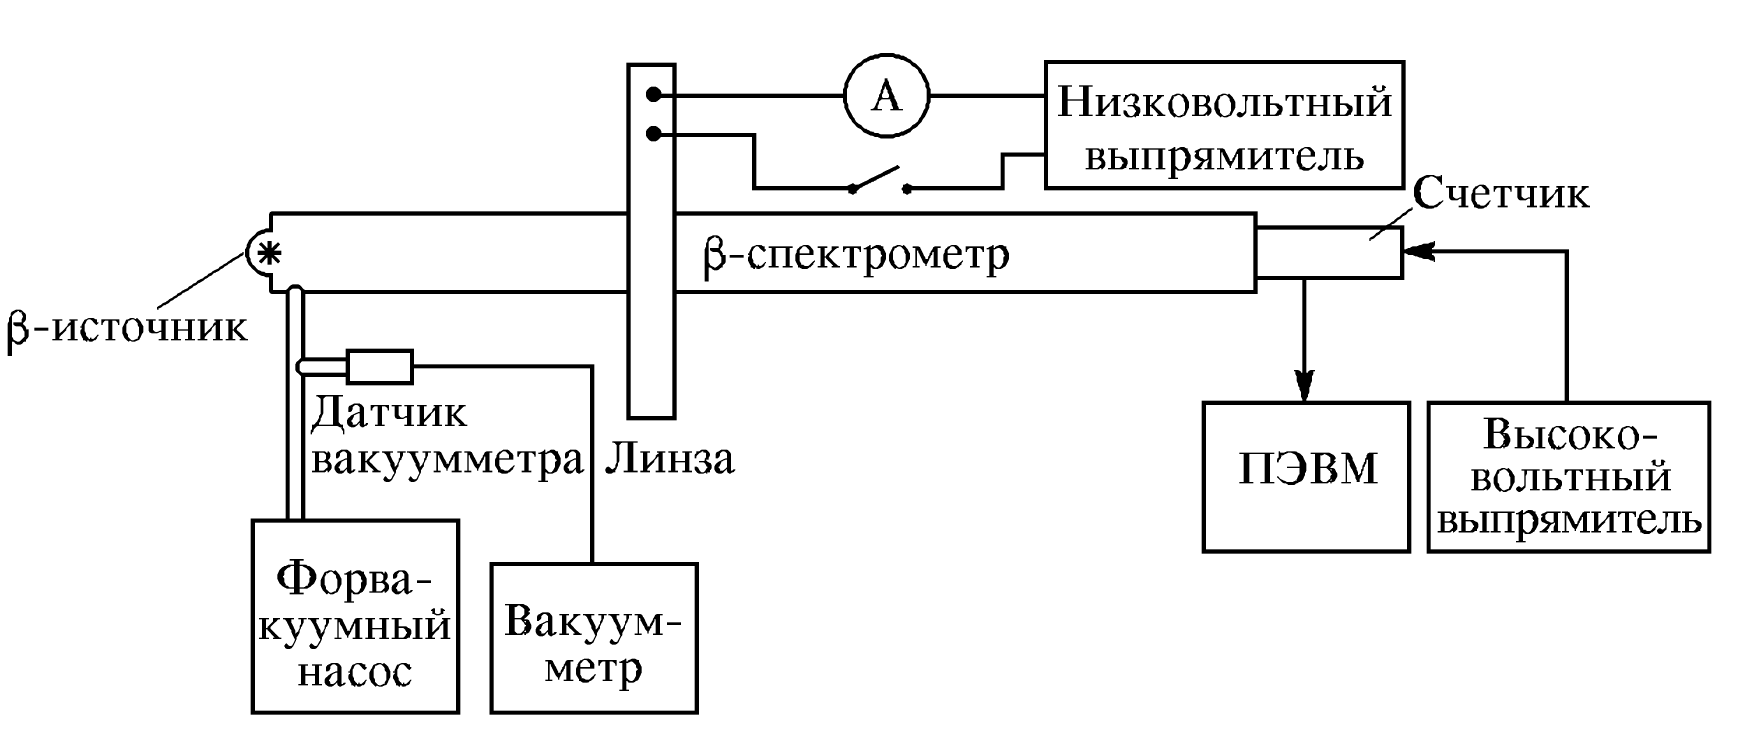
\includegraphics[width=0.48\textwidth]{lab2}
	\caption{слева --- схема $\beta$-спектрометра; справа --- блок-схема установки для изучения спектра}
	\label{pic:scheme}
\end{figure}

В $\beta$-спектрометре установлены диафрагмы для ограничения углов вылета частиц из источника и свинцовый фильтр для защиты от прямого попадания $\gamma$-лучей. 

Число частиц $N$, регистрируемых на установке, равно: $N \approx W \cdot \Delta p_e$, где $\Delta p_e$ - разрешающая способность спектрометра. Дифференцируя выражение для форуса магнитной линзы, получим: $\Delta p_e = \frac{1}{2}\frac{\Delta f}{f}p_e$, то есть $\Delta p_e \propto p_e$. Таким образом, для количества частиц справедлива формула: 

\begin{equation}\label{N}
 N = CW(p_e)p_e 
\end{equation}

Здесь $C$ - некоторая константа.


\section{Выполнение работы}

Откачаем воздух из полости спектрометра, включим вакуумметр. Включим ПЭВМ, формирователь импульсов, питание магнитной линзы и уменьшим ток через неё до нуля. 

Проведём измерение $\beta$-спектра, изменяя ток в магнитной линзе, при каждом значении тока будем измерять число попаданий частиц в детектор за 100 секунд. Далее в таблице будут сразу приведены значения $ N[с^{-1}] = \frac{N'}{t_{100}} $ --- число частиц в единицу времени. Результаты сведем в таблицу \ref{table_1}. 

\textit{Примечание: в таблице погрешности величин указаны в тех же размерностях, что и сами величины.}

\begin{table}[h!]
	\caption{Результаты измерений}
	\begin{center}
		\begin{tabular}{|c|c|c|c|c|c|c|c|c|c|c|c|}
			\hline
			№ & $ I, $ А & $ \sigma_l $, А & $ N, \; с^{-1} $ & $ N - N_ф,  \; с^{-1} $ & $ \sigma_{N-N_ф}$  & $ p, \; кэВ/c $,  & $ \sigma_p \;  $  & $ T $, кэВ & $ \sigma_T $ & $ f, \; с/м^{3/2 } $& $ \sigma_f \;$\\
			\hline
1 & 0 & 0.02 & 0.66 & -0.13 & 0.14 & - & - & - & - & - &- \\
2 & 0.2 & 0.02 & 0.71 & -0.08 & 0.14 & 51 & 5 & 3 & 0 & - & - \\
3 & 0.4 & 0.02 & 0.91 & 0.12 & 0.15 & 103 & 5 & 10 & 1 & 3.322 & 0.118 \\
4 & 0.6 & 0.02 & 0.89 & 0.1 & 0.14 & 154 & 5 & 23 & 1 & 1.651 & 0.118 \\
5 & 0.8 & 0.02 & 0.96 & 0.17 & 0.15 & 206 & 5 & 40 & 1 & 1.398 & 0.118 \\
6 & 1 & 0.02 & 1.37 & 0.58 & 0.16 & 257 & 5 & 61 & 1 & 1.848 & 0.118 \\
7 & 1.2 & 0.02 & 1.78 & 0.99 & 0.17 & 309 & 6 & 86 & 2 & 1.835 & 0.118 \\
8 & 1.4 & 0.02 & 2.4 & 1.61 & 0.19 & 360 & 6 & 114 & 2 & 1.858 & 0.118 \\
9 & 1.7 & 0.02 & 3.52 & 2.73 & 0.22 & 437 & 6 & 161 & 2 & 1.808 & 0.081 \\
10 & 2 & 0.02 & 3.96 & 3.17 & 0.23 & 514 & 6 & 214 & 3 & 1.527 & 0.062 \\
11 & 2.3 & 0.02 & 3.97 & 3.18 & 0.23 & 591 & 7 & 271 & 3 & 1.24 & 0.049 \\
12 & 2.6 & 0.02 & 4.05 & 3.26 & 0.23 & 668 & 7 & 330 & 3 & 1.045 & 0.04 \\
13 & 2.9 & 0.02 & 3.56 & 2.77 & 0.22 & 746 & 7 & 393 & 4 & 0.817 & 0.034 \\
14 & 3.2 & 0.02 & 2.57 & 1.78 & 0.19 & 823 & 8 & 457 & 4 & 0.565 & 0.032 \\
15 & 3.3 & 0.02 & 2.27 & 1.48 & 0.19 & 848 & 8 & 479 & 5 & 0.492 & 0.032 \\
16 & 3.4 & 0.02 & 1.42 & 0.63 & 0.16 & 874 & 8 & 502 & 5 & 0.307 & 0.04 \\
17 & 3.6 & 0.02 & 1.3 & 0.51 & 0.16 & 926 & 8 & 546 & 5 & 0.254 & 0.04 \\
18 & 3.7 & 0.02 & 1 & 0.21 & 0.15 & 951 & 9 & 569 & 5 & 0.156 & 0.055 \\
19 & 3.8 & 0.02 & 1.14 & 0.35 & 0.15 & 977 & 9 & 592 & 5 & 0.194 & 0.043 \\
20 & 3.85 & 0.02 & 1.71 & 0.92 & 0.17 & 990 & 9 & 603 & 5 & 0.308 & 0.029 \\
21 & 3.9 & 0.02 & 2.89 & 2.1 & 0.2 & 1003 & 9 & 614 & 5 & 0.456 & 0.023 \\
22 & 3.95 & 0.02 & 4.42 & 3.63 & 0.24 & 1015 & 9 & 626 & 6 & 0.589 & 0.021 \\
23 & 4 & 0.02 & 5.23 & 4.44 & 0.25 & 1028 & 9 & 637 & 6 & 0.639 & 0.02 \\
24 & 4.1 & 0.02 & 5.11 & 4.32 & 0.25 & 1054 & 9 & 660 & 6 & 0.607 & 0.019 \\
25 & 4.2 & 0.02 & 4.58 & 3.79 & 0.24 & 1080 & 9 & 684 & 6 & 0.549 & 0.019 \\
26 & 4.3 & 0.02 & 4.23 & 3.44 & 0.23 & 1105 & 10 & 707 & 6 & 0.505 & 0.018 \\
27 & 4.33 & 0.02 & 3.38 & 2.59 & 0.21 & 1113 & 10 & 714 & 6 & 0.433 & 0.019 \\
28 & 4.35 & 0.02 & 2.4 & 1.61 & 0.19 & 1118 & 10 & 719 & 6 & 0.339 & 0.02 \\
29 & 4.4 & 0.02 & 2.12 & 1.33 & 0.18 & 1131 & 10 & 730 & 6 & 0.303 & 0.021 \\
30 & 4.5 & 0.02 & 0.9 & 0.11 & 0.15 & 1157 & 10 & 754 & 6 & 0.084 & 0.056 \\
31 & 4.6 & 0.02 & 0.56 & -0.23 & 0.13 & 1183 & 10 & 777 & 7 & - & - \\
32 & 4.8 & 0.02 & 0.54 & -0.25 & 0.13 & 1234 & 10 & 825 & 7 &- & - \\
33 & 5 & 0.02 & 0.32 & -0.47 & 0.12 & 1285 & 11 & 872 & 7 & - & - \\
			\hline
		\end{tabular}
	\end{center}
	\label{table_1}
\end{table}

Измерим фон:
\begin{table}[H]
	\caption{Подсчет фона}
\begin{center}
	\begin{tabular}{|c|c|c|c|c|}
	\hline 
	№ & 1 & 2 & 3 & 4 \\ 
	\hline 
	$ N_ф $ & 0,810 & 0,914 & 0,801 & 0,769 \\ 
	\hline 
	$ \sigma_{N_ф }$ & 0,089 & 0,078 & 0,101 & 0,077 \\ 
	\hline 
\end{tabular}
\end{center} 
\end{table}
По результатам измерений возьмем среднее, т.е. 

\begin{equation}\label{}
N_ф = 0,79 \pm 0,09 \; с^{-1}
\end{equation}

Проведем вычет фона из числа частиц. Погрешность будет вычисляться как

\begin{equation}\label{}
\sigma_{N - N_ф} = \sqrt{\sigma_N^2 + \sigma_{N_ф}^2} = \sqrt{\left( \dfrac{\sqrt{N'}}{t_{100}} \right) ^2 + \sigma_{N_ф}^2} 
\end{equation}  

Погрешность $ \sigma_N $ вычисляется статистически. 

Отложим на графике экспериментальные точки в осях $ I, \; N-N_ф $ и профитируем их функцией 

\begin{equation}\label{}
y(x) = g + a \exp\left( \dfrac{(x - b)^2}{2c^2} \right) + d\x x^2(f - \sqrt{x^2 + e})^2
\end{equation}

Первый член вносит общую поправку значений по $ y $ (обусловленную вычетом фона), второй --- функция Гаусса для конверсионного пика и третий --- спектр \be-распада. Результаты фита сведем в таблицу \ref{fit}.

Важным результатом фита является параметр $ b = (4.122 \pm 0.015) \; А $ --- он показывает, где находится конверсионный пик по оси абсцисс. С его помощью можно найти из \eqref{k} 

\begin{equation}\label{}
k = \dfrac{p_c}{I} \approx 245/c \; кэВ / А
\end{equation}

	\begin{figure}[H]
	\label{graf_4}
	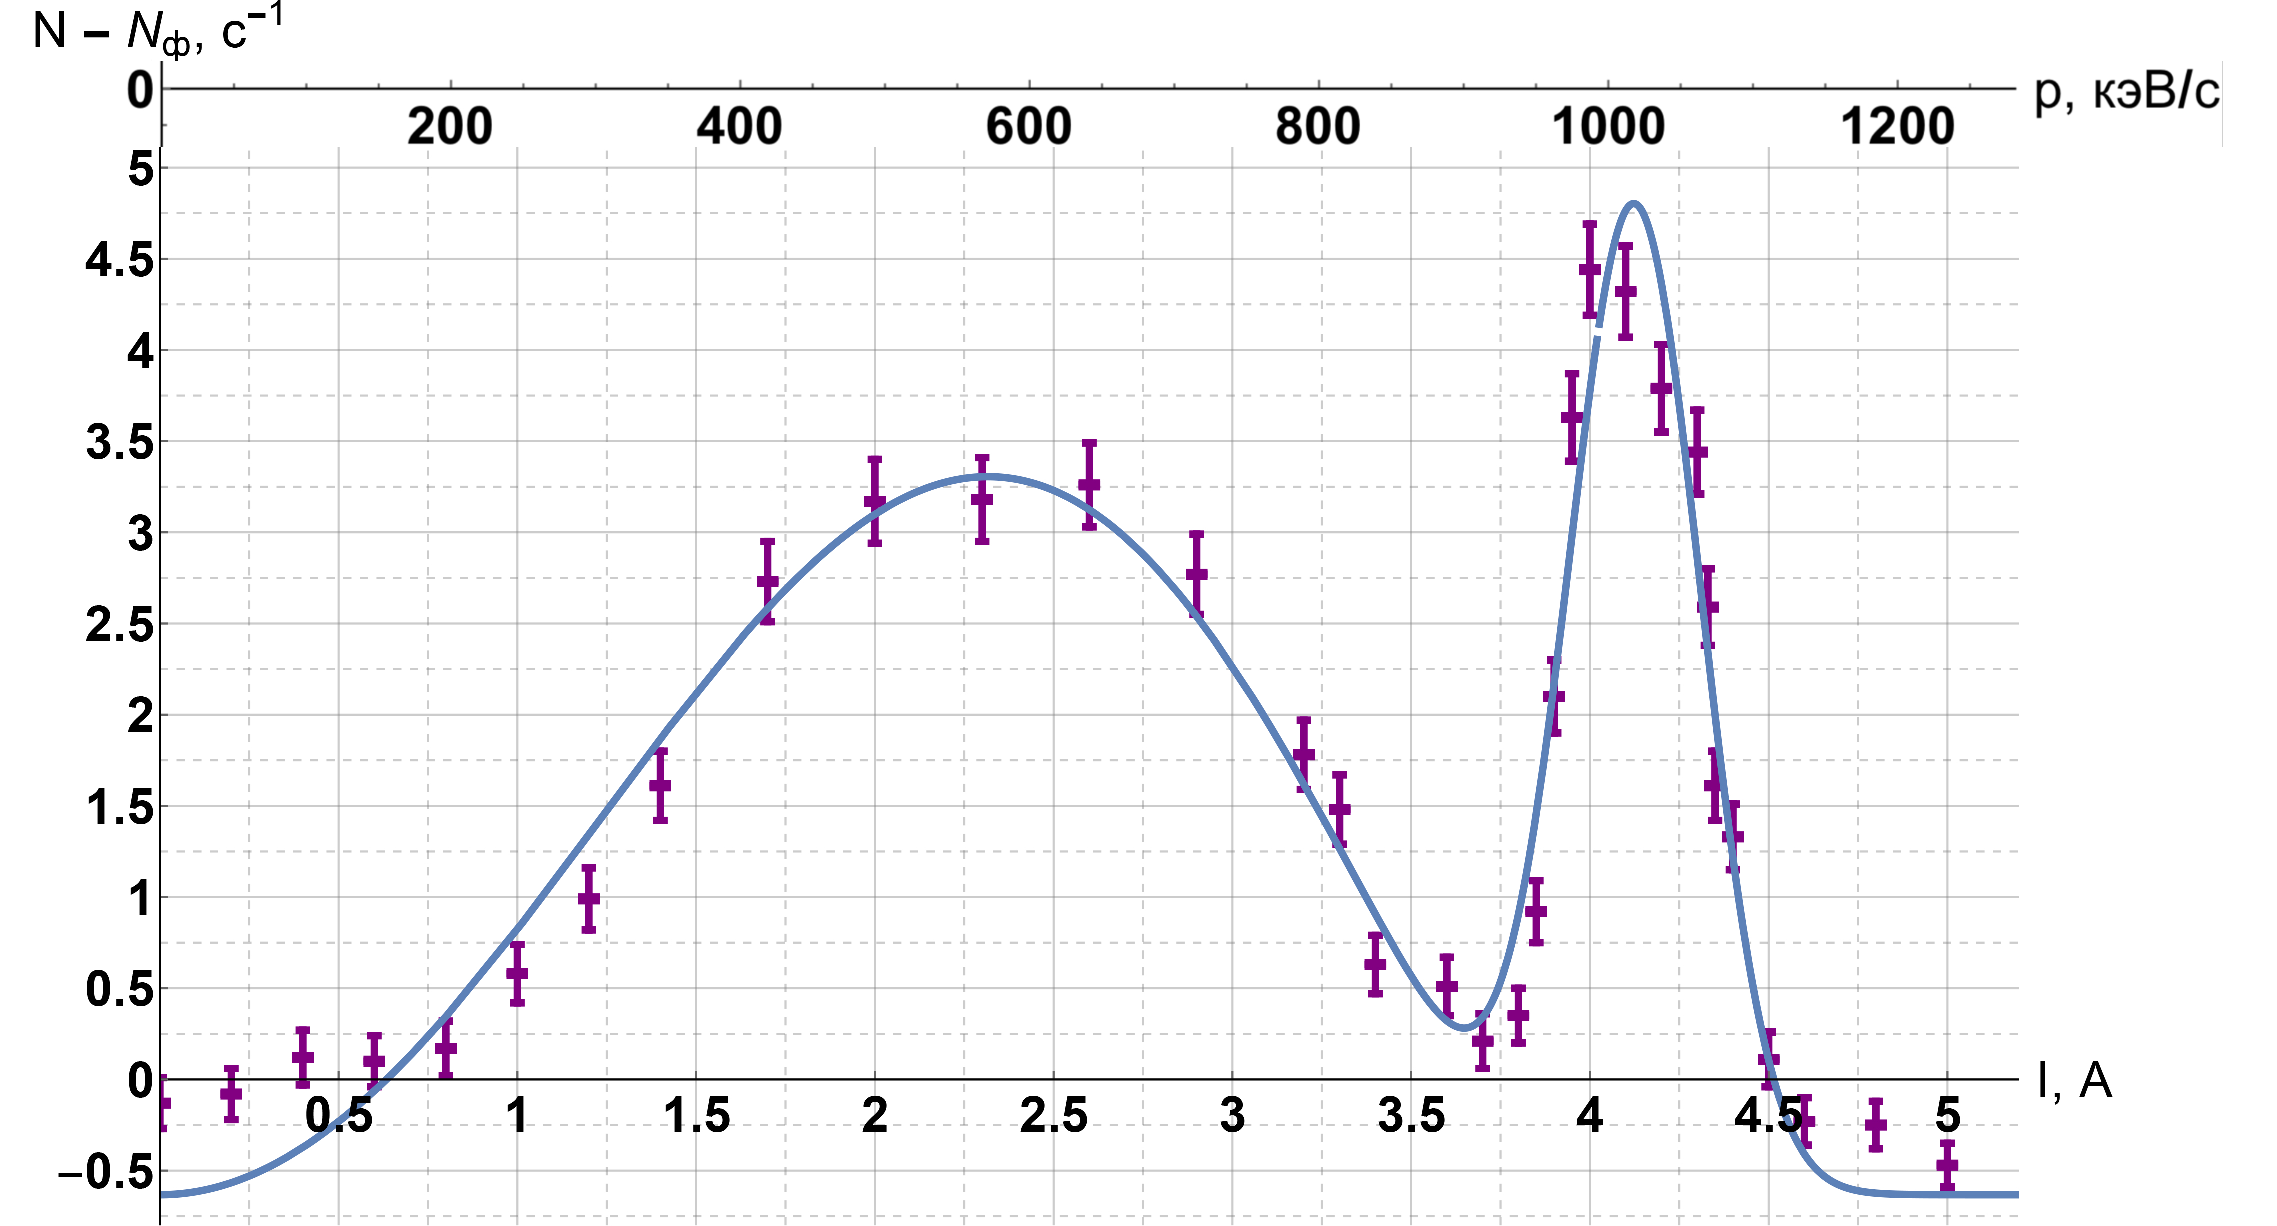
\includegraphics[scale=0.47]{grafp.pdf}
	\caption{Измерение \be-спектра}
\end{figure}

\begin{table}[H]
	\caption{Результаты фита \be-спектра}
	\label{fit}
	\begin{center}
	\begin{tabular}{|c|c|c|}
		\hline
		Параметр & Значение & Ошибка \\
	\hline 
$ a $&5.43 & 0.36 \\
$ b $&4.122 & 0.015 \\
$ c $&0.19 & 0.02\\
$ d $&7.83 & 196.6 \\
$ e $&17.82 & 217.76 \\
$ f $&301.70 & 7766.48 \\
$ g $&-0.63 & 0.27 \\
\hline
$ \chi_\nu $ & \multicolumn{2}{|c|}{3,1}  \\
\hline
\end{tabular}
\end{center} 
\end{table}

Зная конверсионный пик и соответствующие ему импульс $ p_c = 1013 $ кэВ/$ с $ и энергию $ T = 634 $ кэВ, мы можем откалибровать шкалу токов в шкалу импульсов и энергий. Это занесено в таблицу \ref{table_1}.

Теперь подставим в \eqref{dN/dE} формулу \eqref{N}, сокращая обе части на $ \delta  p_e $, мы получаем 

\begin{equation}\label{}
N(p) = \approx p^3 (E_e - E)^2 \te \dfrac{\sqrt{N}}{p^{3/2}} \varpropto T_{max} - T
\end{equation}

Отложив по оси $ y $ величину $ \dfrac{\sqrt{N}}{p^{3/2}} = f $ в таблице \ref{table_1}, а по $ x $ --- кинетическую энергию, мы можем построить график, называемый графиком Ферми-Кюри, и определить по нему $ T_{max} $ --- в этих осях спектр \be-распада описывается прямой, который мы можем профитировать $ y = ax +b $.

	\begin{figure}[H]
	\label{graf_kk}
	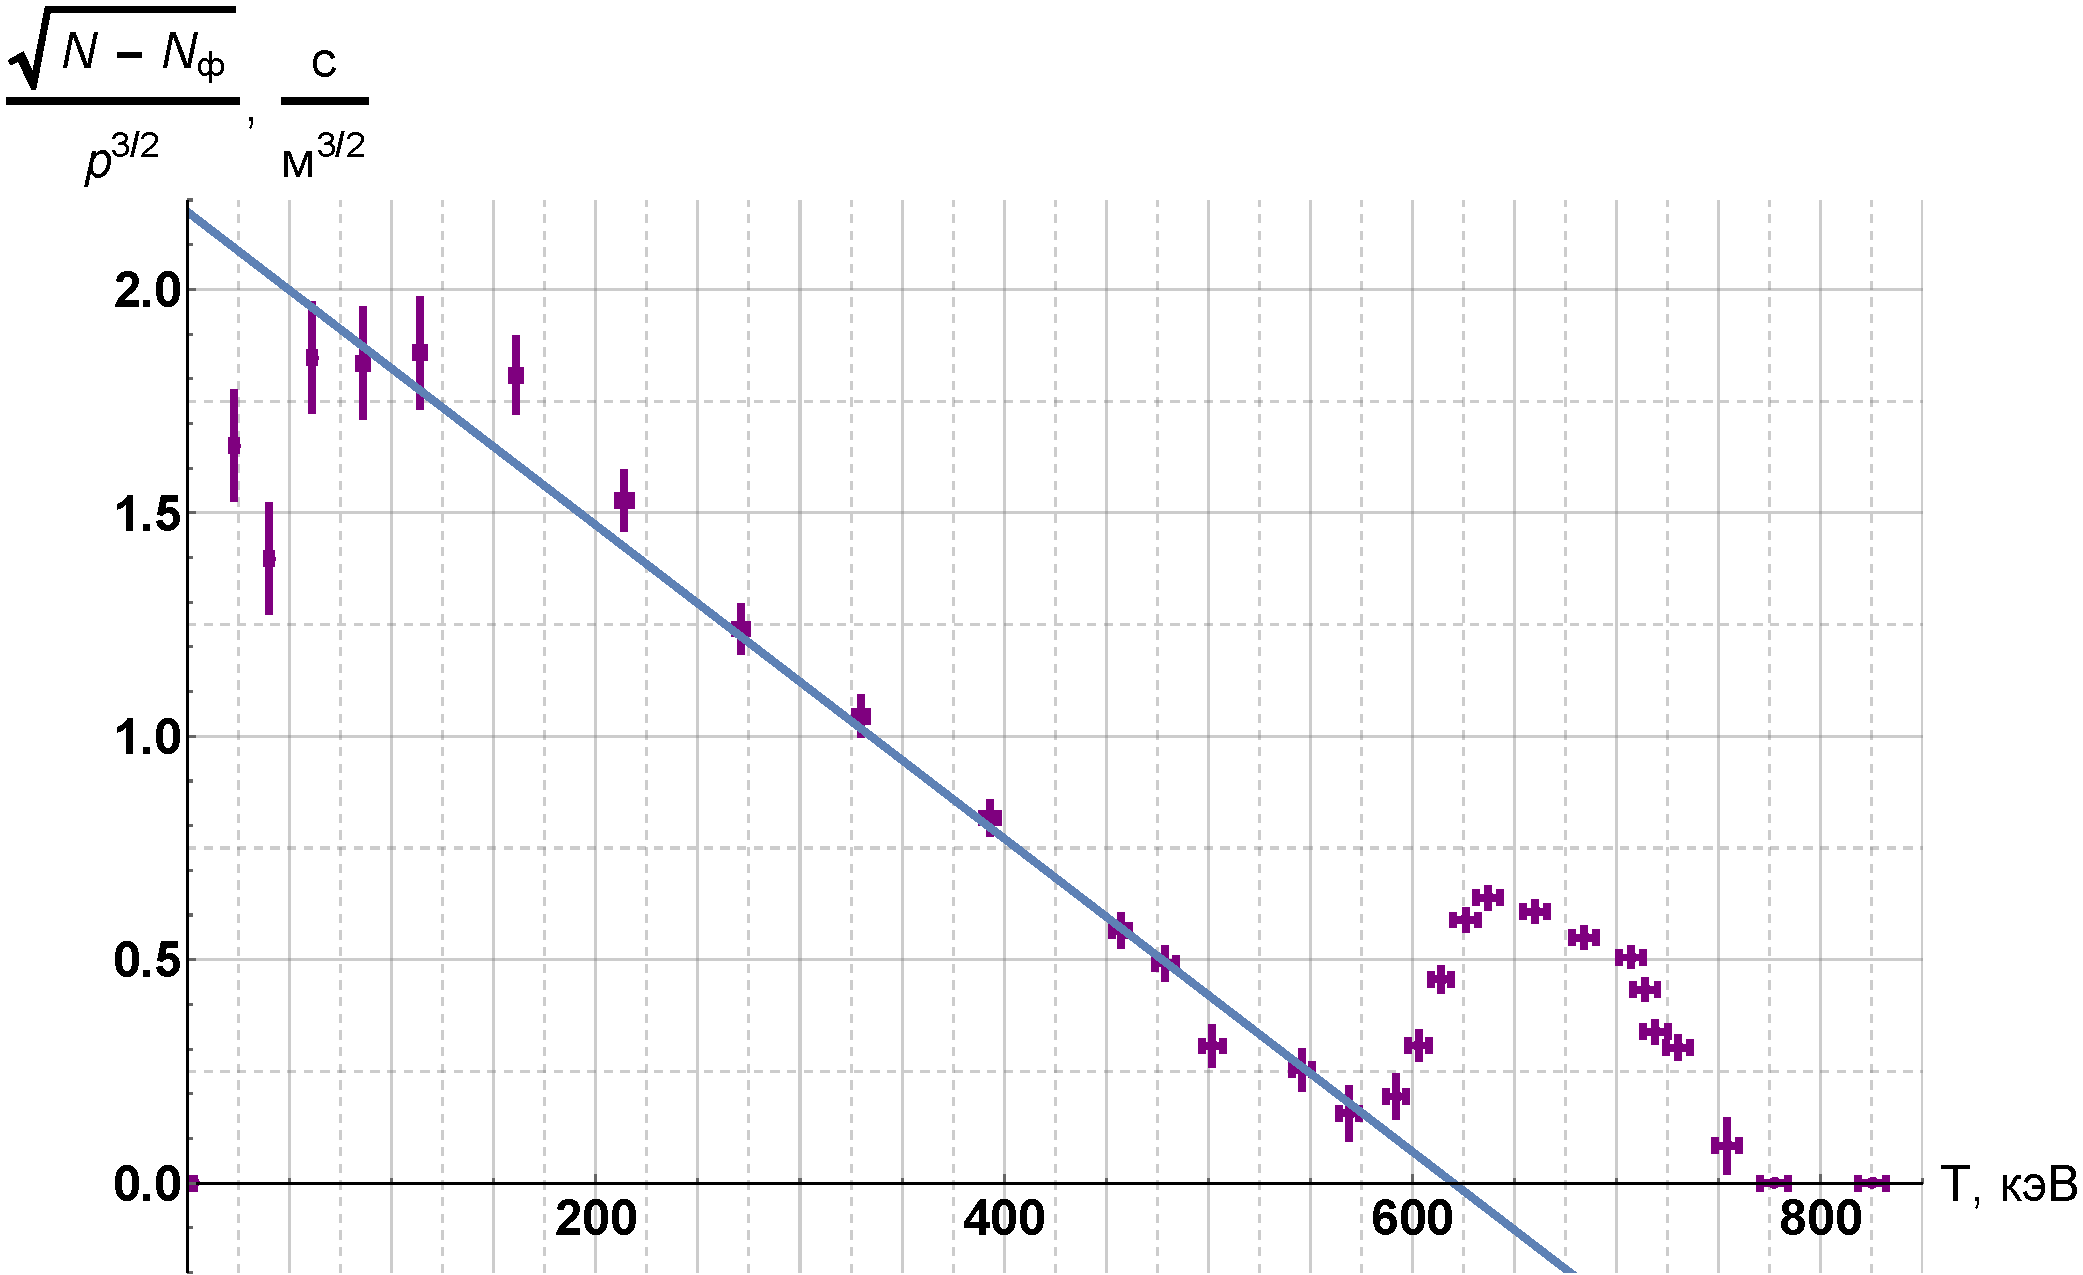
\includegraphics[scale=0.47]{kk.pdf}
	\caption{График Ферми-Кюри}
\end{figure}

В результате фита мы получаем, что при $ y = 0 $ мы можем найти $ T_{max} = \dfrac{b}{-a} \approx (610 \pm 46) \; кэВ $. 

\begin{table}[H]
	\caption{Результаты фита Ферми-Кюри}
	\label{fit_k}
	\begin{center}
		\begin{tabular}{|c|c|c|}
			\hline
			Параметр & Значение & Ошибка \\
			\hline 
			$ b $&2.17 & 0.13 \\
		$ a $ &	-0.0035 & 0.0003 \\
			\hline
			$ \chi_\nu $ & \multicolumn{2}{|c|}{2,1}  \\
			\hline
		\end{tabular}
	\end{center} 
\end{table}

	
	\section{Вывод}
	
	Таким образом, в работе мы изучили спектр \be-распада $  ^{136} Cs $, экспериментальным путем наши конверсионный пик, оценили параметры установки и подсчитали максимальную возможную кинетическую энергию электрона в этом распаде.
	
	
	
\end{document}
